Die Regulierungsbehörde, ein Teil der Bundesnetzagentur (BNetzA), ist eine Bundesoberbehörde mit Sitz in Bonn, welche am 01.01.1998 als Nachfolgerin des Bundesministeriums für Post und Telekommunikation sowie der Deutschen Bundespost gegründet wurde. Die Kontrolle der Einhaltung der gesetzlichen Bestimmungen des Signaturgesetzes ist nur ein Bestandteil der Behörde, welche auch für das Wettbewerbsrecht der Telekommunikationsbranche zuständig ist. Die Hauptaufgaben der BNetzA im Signaturprozess liegt in der Vergabe und Entziehung der Genehmigungen für den Betrieb einer Zertifizierungsstelle, der Kontrolle der Zertifizierungsstellen sowie der Ausstellung eines Zertifikates zur Authentifizierung der Zertifizierungsstelle. \cite{standdeswissens3}\cite{regBeh1}
\begin{figure}[!ht]
    \centering
    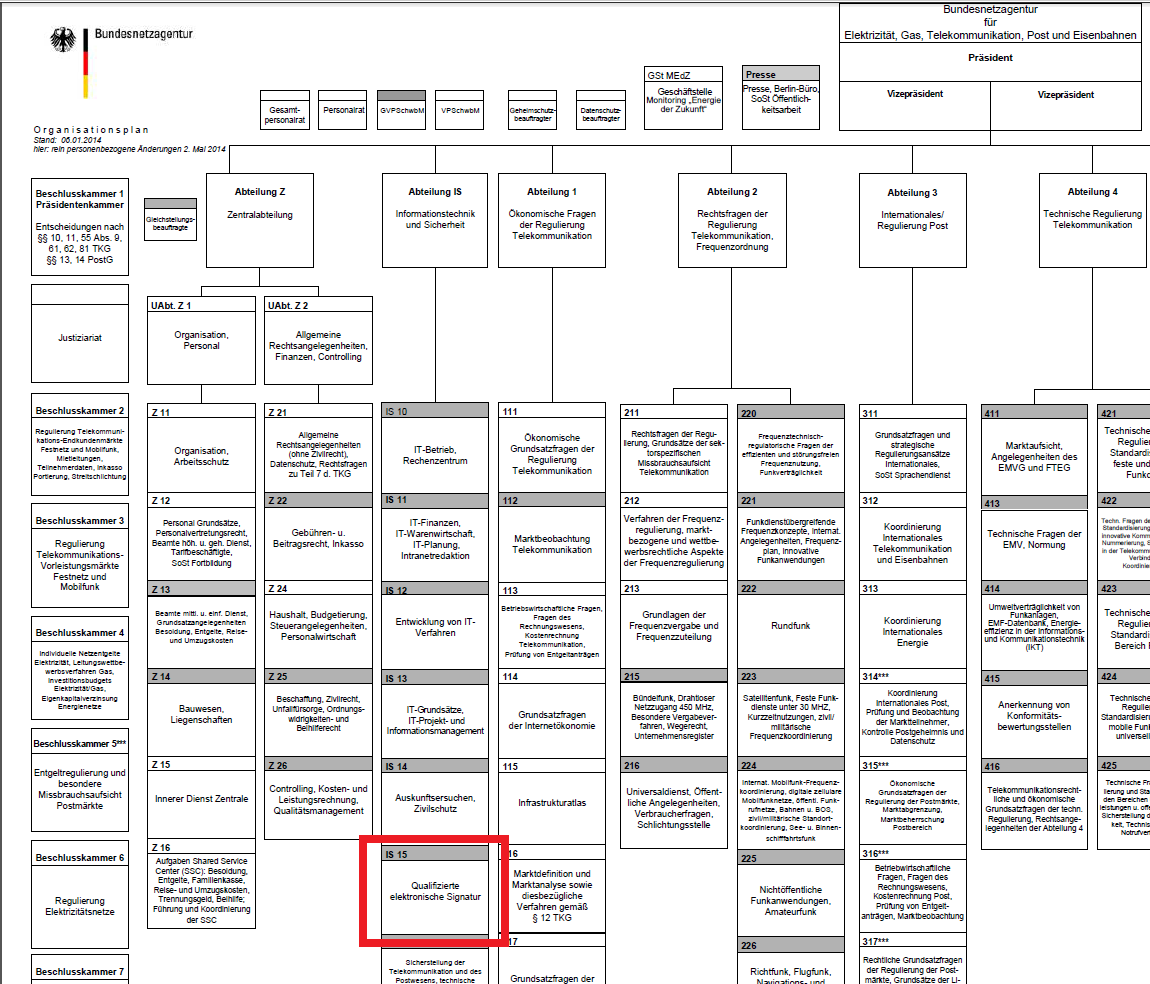
\includegraphics[height=310pt, width=\textwidth]{auszug_orgigram.PNG}
    \caption[Auszug Organigramm Bundesnetzagentur]{\small{Auszug Organigramm Bundesnetzagentur. \cite{BNetzA1}}}
\end{figure}